\documentclass[8pt,a4paper]{article}
\usepackage[utf8]{inputenc}
\usepackage{graphicx}
\graphicspath{ {./images/} }

\usepackage{color}   
\usepackage{hyperref}
\usepackage{listings}
\usepackage[utf8]{inputenc}
\usepackage{amsmath}
\usepackage{amsfonts}
\usepackage{amsthm}
\usepackage{german}

\usepackage[onehalfspacing]{setspace}


\let\stdsection\section
\setlength{\parindent}{0in} 


% Useful packages
\usepackage{amsmath}
\usepackage{graphicx}
\usepackage[colorlinks=true, allcolors=blue]{hyperref}
\title{Neuronale Netze in der Bildverarbeitung Versuch-1}
\author{Julian Schmidt, Vincenz Forkel}

\begin{document}
\maketitle
\newpage
Ziel des ersten Versuchs des Praktikums Neuronale Netze in der Bildverarbeitung im Wintersemester 2021/22 ist es Grundlagen des Aufbaus und der Arbeit mit Neuronalen Netzen kennen zu lernen.\\
Konkret wird hier der MNIST-Datensatz verwendet, für den ein Neuronales Netz darauf trainiert werden soll Ziffern zwischen 0 und 9 zu klassifizieren.\\
Hier für wurde ein Netz der folgenden Architektur gewählt.\\

\begin{center}
    

    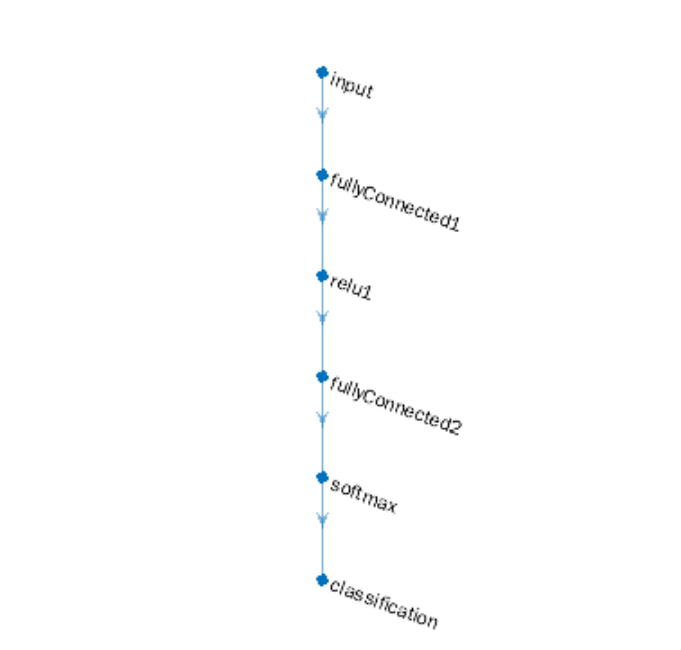
\includegraphics[scale = 0.4]{model.png}
    \caption{Netz Architektur}
\end{center}


Der MNIST (Modified National Institute of Standards and Technology database) ist eine öffentlich verfügbare Datenbank von handgeschriebenen Ziffern.\\
Wobei jede Ziffer als 28 × 28 Pixel großes Graustufen-Bild gespeichert ist.\\

Verwendet wird hierfür die Skript Sprache Matlab.\\

Alle Skripte und Lösungen befinden sich in diesem Github Repository:\\
https://github.com/JulianSchmidt96/MessTechnikPraktikumNN/\\

Im Verlaufe der Praktiumsdurchführung wurden verschiedene Hyperparameter verändert.\\

Mit dem Optimizer Adam lies sich bei einer Trainingsdauer von 30 Epochen eine finale Validierungsgenauigkeit von ca. 98 Prozent erreichen.
\\
Es hat sich eindeutig gezeigt, dass Adam ein genauerer Optimizer als SGDM ist.

Die Lernrate scheint ebenfalls einen großen Einfluss auf die Genauigkeit des Netzes zu haben. um zu schauen wie sich die Genauigkeit des Netzes verbessert hat.\\

Auch wenn sich die Genauigkeit beinahe durchgehend in einem Bereich größer 90 Prozent befindet lässt sich die Genauigkeit immernoch etwas verbessern durch das durchprobieren verschiedener Lernraten.
Hierbei wurden die Lernraten jeweils um den Faktor 10 verändert.\\

Testweise haben wir in einem großem Durchlauf einmal den Lernratenarray so angepasst das wir ca 50 verschiedene Lernraten getestet haben.\\
Hierfür muss lediglich der lernratenarray angepaßt werden, das Skript findet selbstständig die ideale Lernrate.
Zu Beachten ist allerdings, dass hier für eine sehr lange Laufzeit eingeplant werden muss.\\

Wir haben hierfür einmal das Skript über ein Wochenende laufen lassen.

Eine geschickte Anpassung der Minibatch-Größen würde die Trainings-Dauer und somit Gesamtlaufzeit verringern.

Die Ergebnisse haben gezeigt, dass Änderungen der Minibatch-Größe einen direkten Einfluss auf die Laufzeit hat.\\
Beim Testen hat sich gezeigt, dass für verschiedene Minibatch-Größe unterschiedliche Genauigkeiten erreicht wurden.\\
Das liegt allerdings mit hoher Wahrscheinlichkeit da dran, dass jede Prädiktion auf statistischen Größen basiert.\\
Wenn ein Neuronales Netz mehrfach mit exakt gleichen Parametern trainiert wird, ist es  unmöglich immer zu 100 Prozent das gleiche Ergebnis zu erhalten.
\\

Eine deutliche Genauigkeitsverbessserung lies sich durch das hinzufügen der Zeile:\\

\begin{listing}
'Shuffle','every-epoch', ...
\end{listing}
\\
zu den modeloptionen.
\\  , allerdings steigt damit die Laufzeit sehr stark.\\
Die Validationsfrequenz auf einen sehr kleinen Wert zusätzen sorgt ebenfalls für eine erhöhte 
Grundsätzlich lässt sich mit relativ wenig Aufwand eine hohe Genauigkeit in der Vorhersage von Ziffern auf 28x28 Pixel Bilder mit dem MNIST Datensatz erreichen.\\


\end{document}
